\documentclass{article}

\usepackage[utf8]{inputenc}
\usepackage[T1]{fontenc}
\usepackage[spanish]{babel}
\usepackage{times}
\usepackage{wrapfig}
\usepackage{lmodern}
\usepackage{mathtools}
\usepackage{graphicx}
\usepackage[utf8]{inputenc}
\usepackage{color}
\usepackage{hyperref}
\usepackage{fancyhdr,lipsum}


\hypersetup{
    colorlinks=true, %set true if you want colored links
    linktoc=all,     %set to all if you want both sections and subsections linked
    linkcolor=blue,  %choose some color if you want links to stand out
}
\urlstyle{same}

\title{MEDIDAS PREVENTIVAS EN ORDENADORES PORTÁTILES} 
\author{Antonio Muñoz Cubero} 
\date{13 de Noviembre de 2020} 

\begin{document}
  \maketitle 
    \pagenumbering{gobble}
      \pagestyle{fancy}
  
  \newpage
    \tableofcontents
    \lhead[Medidas Preventivas]{Medidas Preventivas}  %cabecera 
    \lfoot[IES Francisco De Los Rios]{IES Francisco De Los Rios} %pie de pagina
  
  \newpage
    \pagenumbering{arabic}

  \newpage
    \section{Introducción} %Esto es la cabecera de un apartado
      En este trabajo vamos a exponer una serie de riesgos y medidas que podemos subrir y deberíamos tomar en caso de que trabajemos con \textbf{ordenadores portátiles.}
      \\\\
      Hoy en día el mundo está en gran parte informatizado, por tanto, gran parte del sector activo de la población trabajo con equipos informáticos y que además gracias a la 
      evolución en dicho sector en los últimos años, podemos trabajar prácticamente en cualquier parte del mundo siempre que dispongamos de conexión a internet y un ordenador.
      Debido a la gran movilidad que necesitamos hoy día, los ordenadores portátiles han avanzado muchísimo, siendo algunos casi más potentes que algunos de sobremesa. Pero, ¿Ha 
      avanzado el sector en cuanto de prevención de risgos al utilizar dicha tecnología?
      \\\\\\\\
      \begin{figure}[h] 
        \centering
        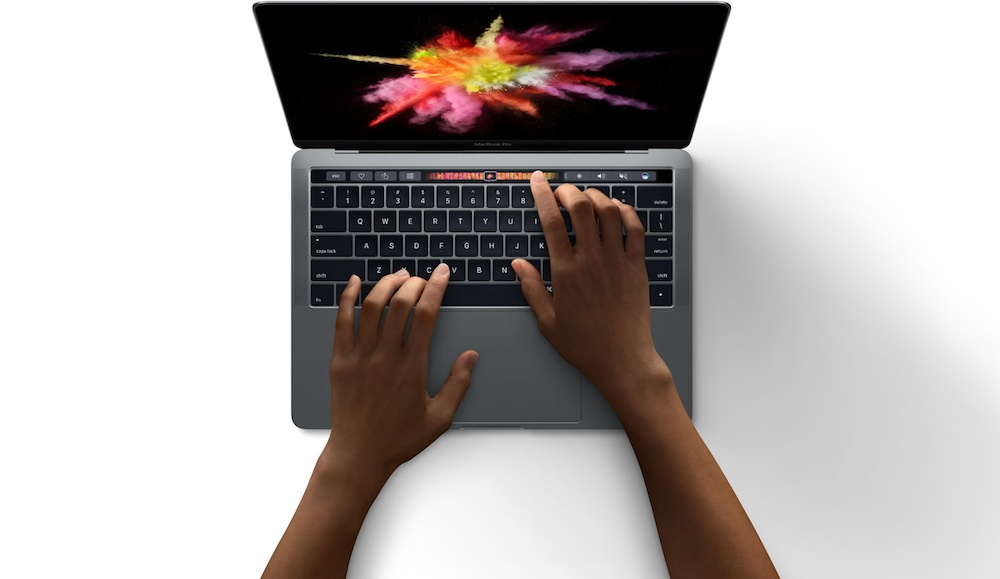
\includegraphics[scale = 0.5]{img/macbook.jpg}
        \caption{MacBook Pro.}
      \end{figure}
  \newpage
    \section{Riesgos}
      \subsection{Factores de riesgo}
      \begin{itemize}
        \item El simple hecho de llevar contigo el portatil ya puede significar un riesgo, puesto que es el desplazamiento de una carga entre las diferentes zonas 
        de trabajo.
        \item Al ser portatil propiamente dicho, se puede improvisar el puesto de trabajo, pero donde muchos ven esto una ventaja, también puede ser un factor de 
        riesgo, ya que puede llevar a una mala postura de forma continuada.
        \item El diseño en si mismo del portatil ya es un factor de riesto, puesto que no permite ajustar de forma conveniente y ergonómica la postira adecuada 
        para trabajar con el, por tanto forzamos cuello, muñecas y cabeza al mismo tiempo.
      \end{itemize}
        
      \begin{figure}[h] 
        \centering
        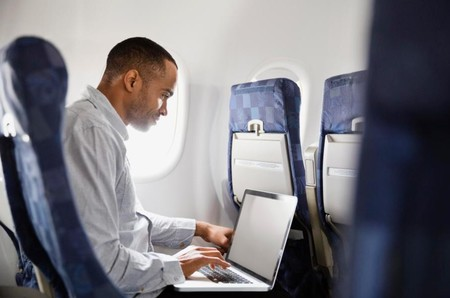
\includegraphics{img/avion.jpg}
        \caption{Trabajando desde un avión.}
      \end{figure}

  \newpage
    \subsection{Identificación de riesgos}
      
      \begin{itemize}
        \item \textbf{Riesgo derivado de la exposición a posturas forzadas o desviación articular originado por la postura de trabajo:} permanecer mucho tiempo sentado en una 
        postura estática hace que se adopten posturas forzadas sobre todo del tronco, el cuello y las extremidades superiores.
        \item \textbf{Fatiga visual:} una iluminación o un contraste de luminarias inadecuado origina deslumbramientos y reflejos en la pantalla. Además, se adoptan posturas 
        forzadas y restringidas para evitar dichos reflejos, como podemos observer en la \textit{Figura 3}.
        \item \textbf{Sobrecarga muscular:} localizada en la zona del cuerpo que soporta el peso del portátil, generalmente en el hombro si se usa un bolso de tipo bandolera, 
        en las extremidades superiores si se usa una maleta con ruedas para arrastrarla o empujarla y la parte alta de la espalda si se usa una mochila.
        \item \textbf{Desviación articular:} como el giro y/o la flexión del cuello, y adaptación continua de la visión a diferentes distancias, luminancias y/o contrastes, 
        por el hecho de tener que situar los documentos fuera de los ángulos visuales.
        \item \textbf{Riesgo derivado de la exposición a movimientos repetitivos realizados durante periodos de tiempos prolongados:} unidos a un entorno de trabajo inadecuado 
        y unos hábitos incorrectos, pueden estar relacionados con lesiones o incomodidades en las manos y las muñecas.
      \end{itemize}
      
      \begin{figure}[h]
        \centering
        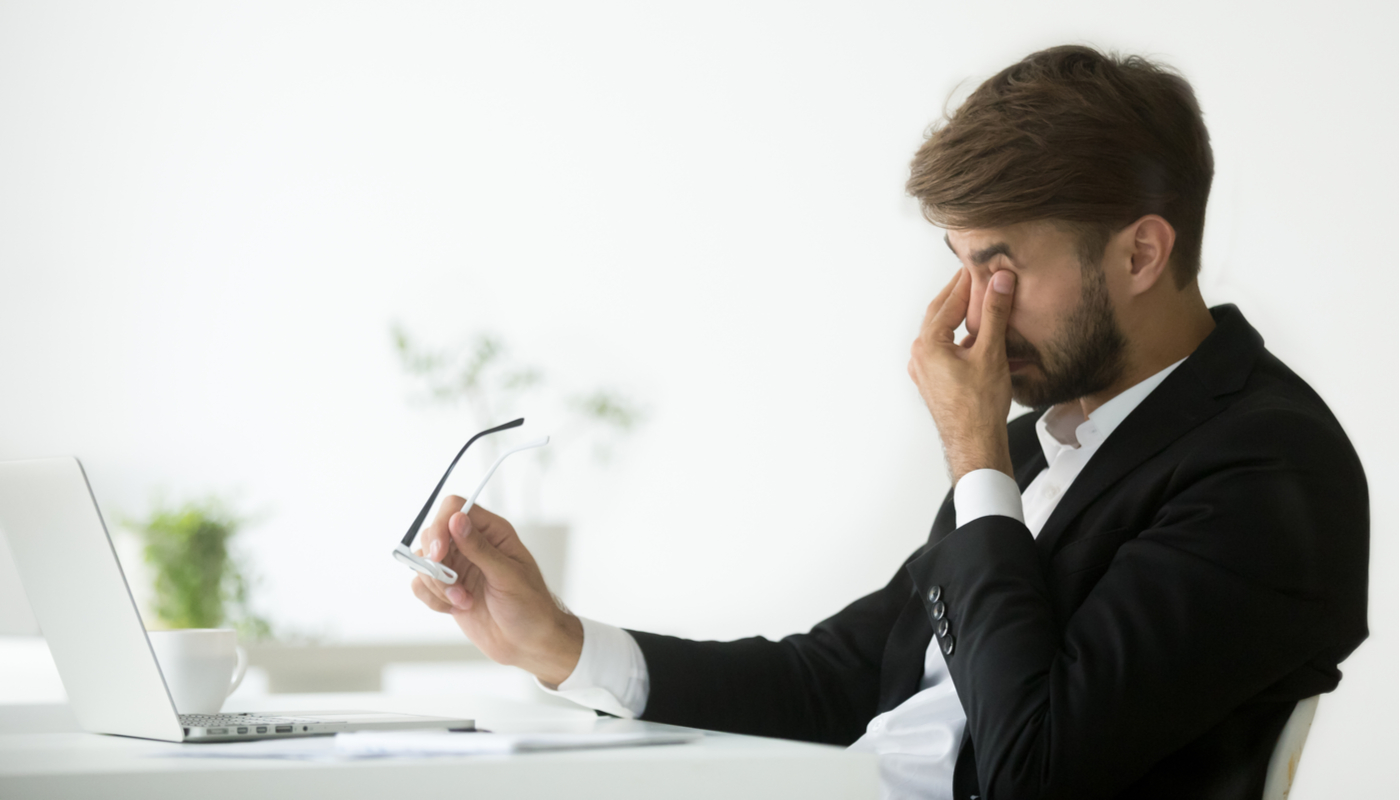
\includegraphics[scale = 0.75]{img/visual.jpg}
        \caption{Fatiga visual en el trabajo.}
      \end{figure}

  \newpage
    \section{Medidas preventivas}
      \subsection{Para el control de la fatiga visual}
        \begin{itemize}
          \item Intentar estar a una distancia de 40cm de la pantalla.
          \item Realizar pausas.
          \item Relajar la mirada, mirando hacia lugares alejados.
          \item Se recomienda equipos con pantallas superiores a 14'.
        \end{itemize}

        \begin{figure}[h]
          \centering
          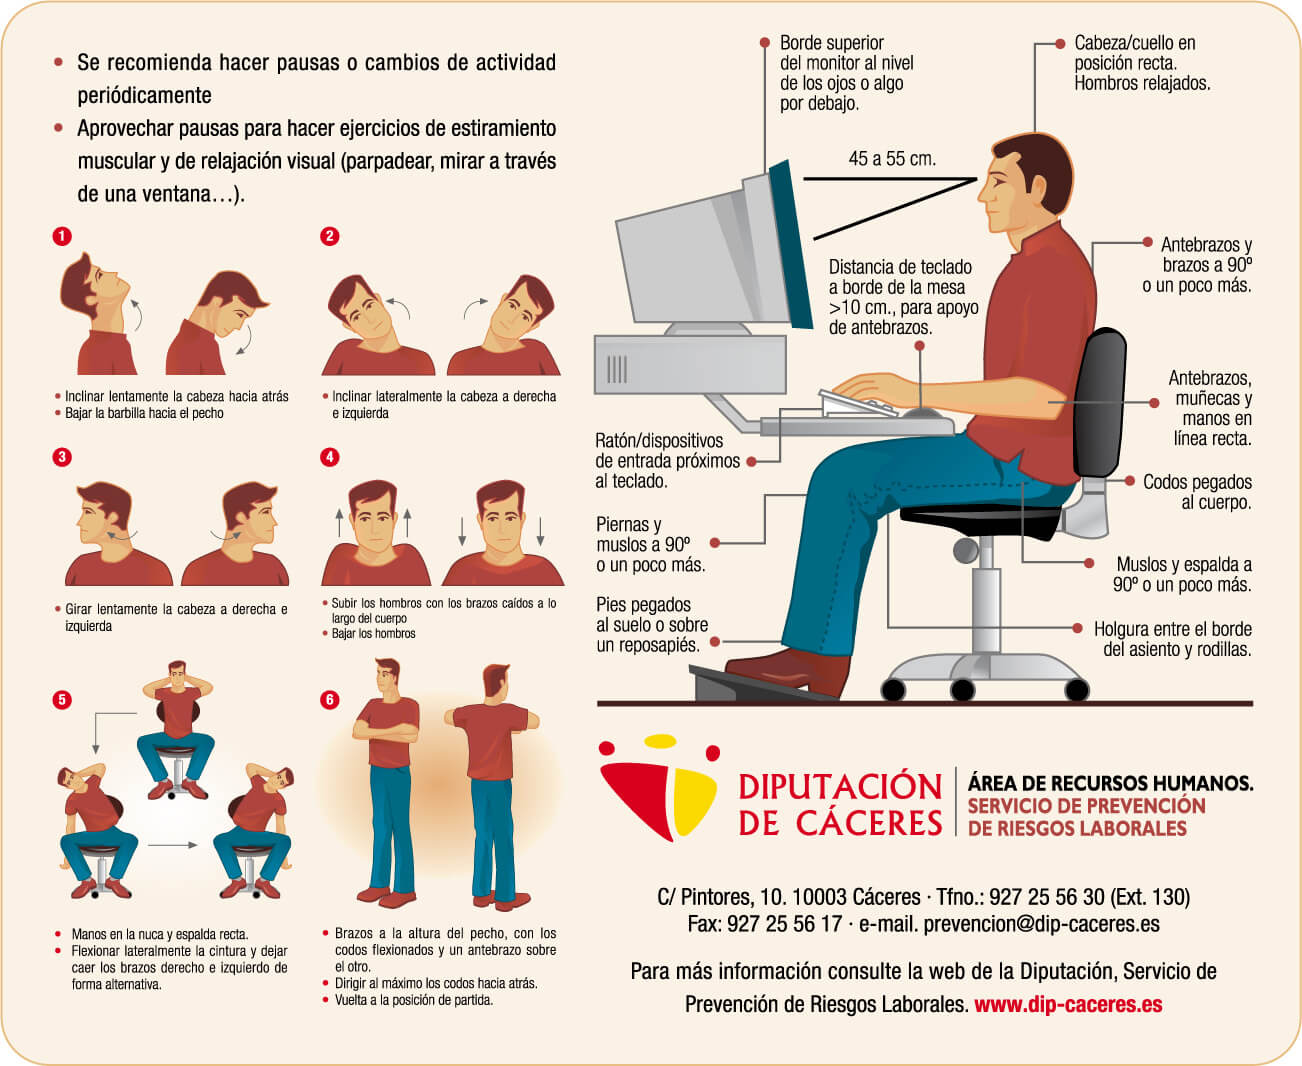
\includegraphics[scale = 0.25]{img/prevencion1.jpg}
          \caption{Ejercicios y posturas para la prevención de riesgos}
        \end{figure}

      \subsection{Para reducir las posturas forzadas y la desviación articular}
        \begin{itemize}
          \item Organizar su área de trabajo de manera que disponga de espacio para las muñecas, trabajar con las muñecas en posición neutras y utilizar reposamuñecas si fuera 
          necesario.
          \item En su puesto de trabajo intertar siempre mantener la espalda apoyada, las piernas tienen que formar un ángulo de 90º, mantener apoyados los pies y las piernas de manera que facilitemos el apoyo lumbar 
          en el asiento y evitemos compresiones en las piernas.
          \item A la hora de trabajar sentarse en posición frontal respecto a la pantalla y, en las tareas que requieran alternar la visualización de la pantalla con la lectura frecuente de documentos 
          impresos, dichos documentos deben estar apoyados en un soporte entre el teclado y la pantalla que permita ubicarlos en unos ángulos visuales o de giro y/o flexión del 
          cuello aceptables.
          \item Hacer descansos frecuentes con ejercicios físicos posturales. Resultan más eficaces las pausas cortas y frecuentes, siempre acompañadas de estiramientos, que las 
          largas y espaciadas.
        \end{itemize}

      \subsection{Para el transporte manual del equipo}
        \begin{itemize}
          \item Cuando se cargue el portátil en un bolso de tipo bandolera, se tiene que cambiar periódicamente el brazo con el que se transporta, de manera que el peso se reparta a ambos lados del cuerpo.
          \item  Escoger los equipos del mercado que ofrecen el peso más reducido, utilizar baterías de larga duración para evitar el transporte de cables y transformador o bien prever la disponibilidad de algún 
          transformador estándar en los centros de trabajo de destino.
        \end{itemize}

      \subsection{Para mejorar las características físicas del entorno de trabajo}
        \begin{itemize}
          \item Los expertos recomiendan usar un teclado y ratón externos, pues los intregrados no son recomendables para largas sesiones de trabajo.
          \item La mesa de trabajo debe tener bordes redondeados y no ser reflectora.
          \item Tener un espacio de trabajo óptimo térmica y acústicamente hablando.
          \item Si tiene que improvisar su lugar de trabajo, intente en la medida de lo posible encontrar un lugar con libertad de movimiento.
        \end{itemize}
    
  \newpage
    \listoffigures
    \section{Referencias}
        \begin{itemize}
          \item \href{https://www.ccoo-servicios.es/archivos/unicaja/PRL_USO_PORTATILES.pdf}{Secretaria Salud Laboral CCOO}
          \item \href{http://www.cen7dias.es/contenido.php?bol=91&id=1913&sec=4}{Confederación de empresarios de Navarra}
          \item \href{https://www.unileon.es/intranet/prevencion/pvd_portatiles.pdf}{Generalitat de CatalunyaDepartament d’Empresai Ocupació}
          \item \href{http://prevencio.gva.es/documents/161660390/169792761/SPRL_DIPRL_12_00++Prevenci%C3%B3n+de+riesgos+laborales+durante+el+uso+del+ordenador+fuera+del+puesto+de+trabajo+habitual/33b7e144-ccaf-4f03-a8d7-b4af4cc2c584}{Servicio de prevención de riesgos de INVASSAT}
        \end{itemize}

    



\end{document}
